% Drawing 148/01-17 -- folder 148, batch 01, archive page 18 (PDF page 19).
% Transcription: au bas de la page, une sphère au crayon : l'équateur, deux méridiens à peine tracés et quatre points marqués sur le contour.
% Kind: pencil sphere with equator, meridians and four points. Method 2 (schematic redraw from the facsimile). Status: ok.
% Notes: Faint pencil. The outline, a slightly tilted oval (doubled on the page, drawn once); the equator, a flattened closed curve fuller at its ends than an ellipse (doubled on the page, drawn once); two meridian strokes from the top of the outline to its bottom, forming a narrow lens left of the centre; four heavy dots on the outline (upper left, upper right, lower left, lower right). A pencil stroke, faint and broken, comes down from above the sphere (it starts some eight units above the crop, under the tetrahedron of 01-16) to a red-brown point just above the equator near the centre, and goes on faintly to a small dark point on the lower front of the equator at the right of centre; a short dark tick on the left meridian at the equator and a small dot at the right of the red-brown point. Redrawn 2026-11-12 (issue 128). 2026-11-13, Claude Opus 5.5, issue 147, overlay check: not compiled (no TeX in the session); the TikZ was rasterised by a local interpreter and laid over the 236 ppi scan rendered at 400 dpi. Redrawn on the ink: the outline fitted as an ellipse on its ink, the equator, the meridians and the long stroke through points moved onto their ink, the dots on the centres of their blots; every stroke lies on its ink to within about one unit, the doubled pencil strokes within the width of the doubling. Changed: the outline is an oval, not a circle; the meridians meet at the top and bottom of the outline; the dots were moved onto their blots (they were up to three units off); the long pencil stroke to the centre, its red-brown point, and the points it reaches are added (the earlier redraw had two small dots there). The two meridians are as faint as the transcription says, and drawn.
% Coordinates: 1 unit = 1 mm = 1/100 of the crop width, y downwards as on the crop (bbox in page fractions: [0.24, 0.62, 0.56, 0.84]).
% Redrawn by Claude (claude-fable-5-2), issue #128, 2026-11-12; not checked by a human; not compiled (no TeX in the session); overlay-checked on the scan by Claude Opus 5.5, issue #147, 2026-11-13, not compiled (no TeX in the session).
% Rights: reproduces part of the work -- behind RENDER_TRANSCRIPTS, never published by itself.
\documentclass[tikz,border=3pt]{standalone}
\usepackage{amsmath,amssymb}
\usetikzlibrary{patterns,arrows.meta}
\tikzset{pencil/.style={black!45}, struck/.style={black!35}, mpt/.style={circle,draw,inner sep=1.3pt}, pt/.style={circle,fill,inner sep=0.9pt}, opt/.style={circle,draw,fill=white,inner sep=1.1pt}, Rd/.style={red!75!black}, Gn/.style={green!45!black}, Br/.style={brown!70!black}}
\begin{document}
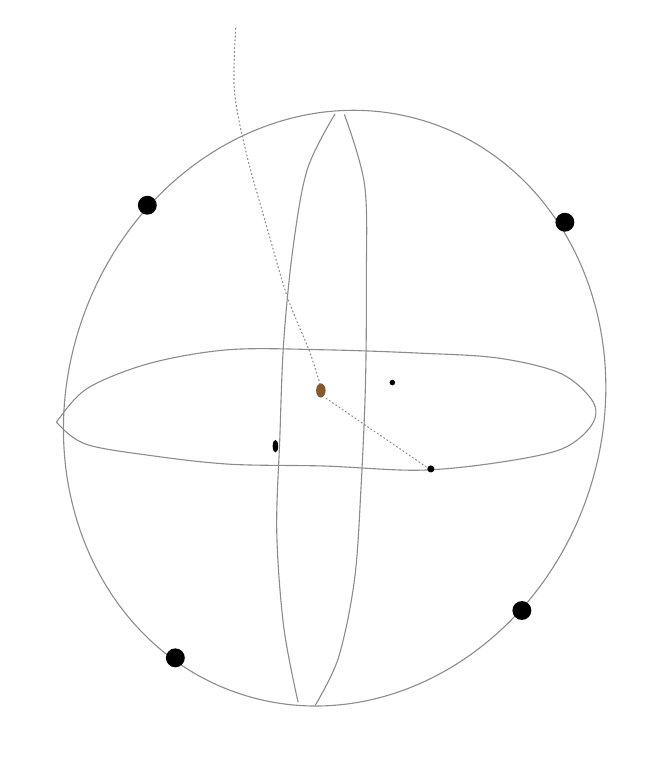
\begin{tikzpicture}[x=1mm,y=-1mm,line cap=round,line join=round,font=\small]
% outline (doubled on the page, drawn once) and equator (doubled, drawn once)
\draw[pencil,rotate around={71.6:(48.28,48.25)}] (48.28,48.25) ellipse [x radius=38.22, y radius=33.99];
\draw[pencil] plot[smooth cycle, tension=0.55] coordinates {(13.4,49.42) (17.07,45.62) (24.9,42.53) (34.93,40.82) (46.99,40.84) (59.01,41.26) (69.05,41.89) (76.98,43.84) (81.08,47.41) (80.93,50.38) (77.14,53.43) (69.09,55.15) (59.04,56.13) (47,55.6) (34.97,55.37) (24.93,54.27) (16.82,52.87) (13.35,50.45)};
% two meridian strokes from the top of the outline to its bottom
\draw[pencil] plot[smooth, tension=0.55] coordinates {(48.32,10.91) (44.81,17.93) (42.97,28.07) (41.8,40.01) (41.32,52) (40.93,64.04) (41.82,76.07) (43.63,85.56)};
\draw[pencil] plot[smooth, tension=0.55] coordinates {(49.53,10.99) (52.09,19.93) (52.31,31.99) (52.2,45) (51.65,57.99) (50.81,69.98) (48.77,79.93) (45.85,85.92)};
% four points on the outline
\fill (24.49,22.48) circle [radius=1.2];
\fill (77.52,24.64) circle [radius=1.2];
\fill (28.05,79.96) circle [radius=1.2];
\fill (72.06,73.95) circle [radius=1.2];
% the pencil stroke coming down from above the sphere to the point near the centre (red-brown), and two small marks
\draw[pencil,densely dotted] plot[smooth, tension=0.55] coordinates {(35.72,0) (35.56,8.03) (37.12,16.1) (39.6,25) (42.26,34.07) (45.04,40.92) (46.5,45.46)};
\fill[Br] (46.53,46.01) ellipse [x radius=0.6, y radius=0.9];
\fill (40.76,53.08) ellipse [x radius=0.35, y radius=0.8];
\fill (55.61,45) circle [radius=0.35];
\draw[pencil,densely dotted] (47.2,47) -- (60.2,55.9);
\fill (60.5,55.97) circle [radius=0.45];
\end{tikzpicture}
\end{document}
